\definecolor{magenta}{HTML}{EB588F}                                          % Linie S1
\newcommand{\mgt}[1]{\cellcolor{magenta}\textcolor{white}{\textbf{#1}}}
\definecolor{darkgreen}{HTML}{047939}                                        % Linien S2, S25
\newcommand{\dgr}[1]{\cellcolor{darkgreen}\textcolor{white}{\textbf{#1}}}
\definecolor{enzianblaus}{HTML}{026597}                                      % Linie S3
\newcommand{\ebs}[1]{\cellcolor{enzianblaus}\textcolor{white}{\textbf{#1}}}
\definecolor{enzianblau}{cmyk}{1.00,0.60,0.00,0.20}                          % Linie U8
\newcommand{\ebl}[1]{\cellcolor{enzianblau}\textcolor{white}{\textbf{#1}}}
\definecolor{lightbrown}{HTML}{AA3C1F}                                       % Linien S41, S42
\newcommand{\lbr}[1]{\cellcolor{lightbrown}\textcolor{white}{\textbf{#1}}}
\newcommand{\lbx}[1]{\colorbox{lightbrown}{\textcolor{white}{\textbf{#1}}}}
\colorlet{mbrown}{lightbrown!80}                                             % Linien S45, S46, S47
\newcommand{\mbr}[1]{\cellcolor{mbrown}\textcolor{white}{\textbf{#1}}}
\newcommand{\mbx}[1]{\colorbox{mbrown}{\textcolor{white}{\textbf{#1}}}}
\definecolor{pastellorangs}{HTML}{EA561C}                                    % Linie S5
%\definecolor{pastellorange}{cmyk}{0.00,0.55,1.00,0.00}                       % Linien S5, U9, Metro-Logo
\newcommand{\pos}[1]{\cellcolor{pastellorangs}\textcolor{white}{\textbf{#1}}}
\newcommand{\pob}[1]{\colorbox{pastellorangs}{\textcolor{white}{\textbf{#1}}}}
\definecolor{pastellorange}{HTML}{F47920}                                    % Linie U9, Metro-Logo
\newcommand{\por}[1]{\cellcolor{pastellorange}\textcolor{white}{\textbf{#1}}}
\newcommand{\pox}[1]{\colorbox{pastellorange}{\textcolor{white}{\textbf{#1}}}}
\definecolor{blaulila}{cmyk}{0.55,0.65,0.00,0.05}                            % Linie U6
\newcommand{\bli}[1]{\cellcolor{blaulila}\textcolor{white}{\textbf{#1}}}
\definecolor{blaulilas}{HTML}{764D9A}                                        % Linien S7, S75
\newcommand{\bls}[1]{\cellcolor{blaulilas}\textcolor{white}{\textbf{#1}}}
\definecolor{hellgruen}{HTML}{4FA433}                                        % Linien S8, S85
\newcommand{\hgr}[1]{\cellcolor{hellgruen}\textcolor{white}{\textbf{#1}}}
\definecolor{rehbraun}{cmyk}{0.55,0.80,0.90,0.10}                            % Linien S9, U5
\newcommand{\rbr}[1]{\cellcolor{rehbraun}\textcolor{white}{\textbf{#1}}}
\definecolor{gelbgruen}{cmyk}{0.70,0.00,1.00,0.10}                           % Linie U1
\newcommand{\ggr}[1]{\cellcolor{gelbgruen}\textcolor{white}{\textbf{#1}}}
\colorlet{mgreen}{gelbgruen!40}                                              % umsteigen
\newcommand{\ggn}[1]{\cellcolor{mgreen}\textcolor{black}{#1}}
\definecolor{blutorange}{cmyk}{0.00,0.85,1.00,0.00}                          % Linie U2
\newcommand{\bor}[1]{\cellcolor{blutorange}\textcolor{white}{\textbf{#1}}}
\definecolor{tuerkisgruen}{cmyk}{1.00,0.30,0.80,0.00}                        % Linie U3
\newcommand{\tgr}[1]{\cellcolor{tuerkisgruen}\textcolor{white}{\textbf{#1}}}
\definecolor{verkehrsgelb}{cmyk}{0.00,0.05,1.00,0.00}                        % Linie U4, BVG-Logo
\newcommand{\vgb}[1]{\cellcolor{verkehrsgelb}\textbf{#1}}
\definecolor{lichtblau}{cmyk}{0.80,0.20,0.00,0.00}                           % Linie U7, Fähre-Logo
\newcommand{\lbl}[1]{\cellcolor{lichtblau}\textcolor{white}{\textbf{#1}}}
\newcommand{\lbb}[1]{\cellcolor{lichtblau}\textcolor{black}{\textbf{#1}}}
\definecolor{verkehrsblau}{cmyk}{1.00,0.50,0.00,0.10}                        % U-Bahn-Logo
\newcommand{\vbl}[1]{\cellcolor{verkehrsblau}\textcolor{white}{\textbf{#1}}}
\definecolor{verkehrsrot}{cmyk}{0.00,1.00,1.00,0.00}                         % Tram-Logo
\newcommand{\vrd}[1]{\cellcolor{verkehrsrot}\textcolor{white}{\textbf{#1}}}
\newcommand{\bfr}[1]{\textcolor{verkehrsrot}{\textbf{#1}}}
\definecolor{verkehrspurpur}{HTML}{901E78}
%\definecolor{verkehrspurpur}{cmyk}{0.40,1.00,0.00,0.00}                      % Bus-Logo
\newcommand{\vpp}[1]{\cellcolor{verkehrspurpur}\textcolor{white}{\textbf{#1}}}
\newcommand{\bfp}[1]{\textcolor{verkehrspurpur}{\textbf{#1}}}
\definecolor{zgrau}{rgb}{0.83,0.83,0.83}                                     % hellgrau
\colorlet{lgrau}{zgrau!60}
\definecolor{bahnrot}{rgb}{0.6745,0.1961,0.2314}                             % DB-Logo
\newcommand{\brd}[1]{\cellcolor{bahnrot}\textcolor{white}{\textbf{#1}}}
\newcommand{\bfb}[1]{\textcolor{bahnrot}{\textbf{#1}}}
\definecolor{schiefergrau}{cmyk}{0.1875,0.00,0.00,1.00}                      % Nachtlinien
\newcommand{\sgr}[1]{\cellcolor{schiefergrau}\textcolor{white}{\textbf{#1}}}
\definecolor{ral-gruen}{rgb}{0.3882,0.8843,0.3365}                           % S-Bahnhöfe
\newcommand{\rgr}[1]{\cellcolor{ral-gruen}\textcolor{white}{\bfseries #1}}
\newcommand{\rgs}[1]{\cellcolor{ral-gruen}{\bfseries #1}}
\xdefinecolor{sgruen}{rgb}{0.2601,0.5925,0.2255}
\newcommand{\sge}[1]{\cellcolor{sgruen}\textcolor{white}{\bfseries #1}}
\definecolor{ral-rot}{RGB}{255,139,141}                             % S+U-Bahnhöfe
\newcommand{\rrd}[1]{\cellcolor{ral-rot}\textcolor{white}{\bfseries #1}}
\colorlet{tbl-rot}{ral-rot!50}
\colorlet{tbl-blau}{cyan!50}
\colorlet{tbl-gruen}{ral-gruen!50}
\colorlet{tbl-yellow}{yellow!50}
% Symbole für Regionalexpresslinien
\definecolor{rei}{HTML}{ED1C24}
\newcommand{\rea}[1]{\cellcolor{rei}{\textcolor{white}{\bfseries #1}}}
\newcommand{\reeins}{\colorbox{rei}{\textcolor{white}{\bfseries RE1}}}
\definecolor{reii}{HTML}{FDD205}
\newcommand{\reb}[1]{\cellcolor{reii}{\textcolor{black}{\bfseries #1}}}
\newcommand{\rezwei}{\colorbox{reii}{\textcolor{black}{\bfseries RE2}}}
\definecolor{reiii}{HTML}{F46717}
\newcommand{\rec}[1]{\cellcolor{reiii}{\textcolor{white}{\bfseries #1}}}
\newcommand{\redrei}{\colorbox{reiii}{\textcolor{white}{\bfseries RE3}}}
\definecolor{reiv}{HTML}{94244D}
\newcommand{\rdd}[1]{\cellcolor{reiv}{\textcolor{white}{\bfseries #1}}}
\newcommand{\revier}{\colorbox{reiv}{\textcolor{white}{\bfseries RE4}}}
\definecolor{rev}{HTML}{156AB8}
\newcommand{\ree}[1]{\cellcolor{rev}{\textcolor{white}{\bfseries #1}}}
\newcommand{\refuenf}{\colorbox{rev}{\textcolor{white}{\bfseries RE5}}}
\definecolor{revi}{HTML}{DD4DAF}
\newcommand{\rff}[1]{\cellcolor{revi}{\textcolor{white}{\bfseries #1}}}
\newcommand{\resechs}{\colorbox{revi}{\textcolor{white}{\bfseries RE6}}}
\definecolor{revii}{HTML}{108449}
\newcommand{\reg}[1]{\cellcolor{revii}{\textcolor{white}{\bfseries #1}}}
\newcommand{\resieben}{\colorbox{revii}{\textcolor{white}{\bfseries RE7}}}
\newcommand{\resechssechs}{\colorbox{black}{\textcolor{white}{\bfseries RE66}}}
\newcommand{\redef}[1]{\colorbox{bahnrot}{\textcolor{white}{\bfseries RE#1}}}
\newcommand{\renr}[1]{%
 \begin{switch}{#1}%
  \case{1}{\reeins}%
  \case{2}{\rezwei}%
  \case{3}{\redrei}%
  \case{4}{\revier}%
  \case{5}{\refuenf}%
  \case{6}{\resechs}%
  \case{7}{\resieben}%
  \case{66}{\resechssechs}%
%  \redef{#1}%
 \end{switch}%
}%
% Symbole für Regionalbahnlinien
\definecolor{rbx}{HTML}{55B831}
\newcommand{\rba}[1]{\cellcolor{rbx}{\textcolor{white}{\bfseries #1}}}
\newcommand{\rbeinsnull}{\colorbox{rbx}{\textcolor{white}{\bfseries RB10}}}
\definecolor{rbxii}{HTML}{A0138E}
\newcommand{\rbb}[1]{\cellcolor{rbxii}{\textcolor{white}{\bfseries #1}}}
\newcommand{\rbeinszwei}{\colorbox{rbxii}{\textcolor{white}{\bfseries RB12}}}
\definecolor{rbxiii}{HTML}{F67C13}
\newcommand{\rbc}[1]{\cellcolor{rbxiii}{\textcolor{white}{\bfseries #1}}}
\newcommand{\rbeinsdrei}{\colorbox{rbxiii}{\textcolor{white}{\bfseries RB13}}}
\definecolor{rbxiv}{HTML}{A0138E}
\newcommand{\rbeinsvier}{\colorbox{rbxiv}{\textcolor{white}{\bfseries RB14}}}
\definecolor{rbxx}{HTML}{108449}
\newcommand{\rbzweinull}{\colorbox{rbxx}{\textcolor{white}{\bfseries RB20}}}
\definecolor{rbxxi}{HTML}{9378B5}
\newcommand{\rbd}[1]{\cellcolor{rbxxi}{\textcolor{white}{\bfseries #1}}}
\newcommand{\rbzweieins}{\colorbox{rbxxi}{\textcolor{white}{\bfseries RB21}}}
\definecolor{rbxxii}{HTML}{3A9FDF}
\newcommand{\rbe}[1]{\cellcolor{rbxxii}{\textcolor{white}{\bfseries #1}}}
\newcommand{\rbzweizwei}{\colorbox{rbxxii}{\textcolor{white}{\bfseries RB22}}}
\definecolor{rbxxiii}{HTML}{A0138E}
\newcommand{\rbzweidrei}{\colorbox{rbxxiii}{\textcolor{white}{\bfseries RB23}}}
\definecolor{rbxxiv}{HTML}{775FB0}
\newcommand{\rbg}[1]{\cellcolor{rbxxiv}{\textcolor{white}{\bfseries #1}}}
\newcommand{\rbzweivier}{\colorbox{rbxxiv}{\textcolor{white}{\bfseries RB24}}}
\definecolor{rbxxv}{HTML}{2785D0}
\newcommand{\rbh}[1]{\cellcolor{rbxxv}{\textcolor{white}{\bfseries #1}}}
\newcommand{\rbzweifuenf}{\colorbox{rbxxv}{\textcolor{white}{\bfseries RB25}}}
\definecolor{rbxxvi}{HTML}{01A998}
\newcommand{\rbi}[1]{\cellcolor{rbxxvi}{\textcolor{white}{\bfseries #1}}}
\newcommand{\rbzweisechs}{\colorbox{rbxxvi}{\textcolor{white}{\bfseries RB26}}}
\definecolor{rbxxvii}{HTML}{ED1C24}
\newcommand{\rbzweisieben}{\colorbox{rbxxvii}{\textcolor{white}{\bfseries RB27}}}
\definecolor{rbxxxiii}{HTML}{ED1C24}
\newcommand{\rbdreidrei}{\colorbox{rbxxxiii}{\textcolor{white}{\bfseries RB33}}}
\definecolor{rbxxxvi}{HTML}{A64C35}
\newcommand{\rbj}[1]{\cellcolor{rbxxxvi}{\textcolor{white}{\bfseries #1}}}
\newcommand{\rbdreisechs}{\colorbox{rbxxxvi}{\textcolor{white}{\bfseries RB36}}}
\definecolor{rblv}{HTML}{F46717}
\newcommand{\rbfuenffuenf}{\colorbox{rblv}{\textcolor{white}{\bfseries RB55}}}
\newcommand{\rbdef}[1]{\colorbox{Gray}{\textcolor{white}{\bfseries RB#1}}}
\newcommand{\rbnr}[1]{%
 \begin{switch}{#1}%
  \case{10}{\rbeinsnull}%
  \case{12}{\rbeinszwei}%
  \case{13}{\rbeinsdrei}%
  \case{14}{\rbeinsvier}%
  \case{20}{\rbzweinull}%
  \case{21}{\rbzweieins}%
  \case{22}{\rbzweizwei}%
  \case{23}{\rbzweidrei}%
  \case{24}{\rbzweivier}%
  \case{25}{\rbzweifuenf}%
  \case{26}{\rbzweisechs}%
  \case{27}{\rbzweisieben}%
  \case{33}{\rbdreidrei}%
  \case{55}{\rbfuenffuenf}%
%  \rbdef{#1}%
 \end{switch}%
}%
% Symbole für S-Bahnlinien
\newcommand{\seins}{\colorbox{magenta}{\textcolor{white}{\bfseries S1}}}
\newcommand{\szwei}{\colorbox{darkgreen}{\textcolor{white}{\bfseries S2}}}
\newcommand{\szweifuenf}{\colorbox{darkgreen}{\textcolor{white}{\bfseries S25}}}
\newcommand{\szweisechs}{\colorbox{darkgreen}{\textcolor{white}{\bfseries S26}}}
\newcommand{\sdrei}{\colorbox{enzianblau}{\textcolor{white}{\bfseries S3}}}
\newcommand{\sviereins}{\colorbox{lightbrown}{\textcolor{white}{\bfseries S41}}}
\newcommand{\svierzwei}{\colorbox{lightbrown}{\textcolor{white}{\bfseries S42}}}
\newcommand{\svierfuenf}{\colorbox{lightbrown}{\textcolor{white}{\bfseries S45}}}
\newcommand{\sviersechs}{\colorbox{lightbrown}{\textcolor{white}{\bfseries S46}}}
\newcommand{\sviersieben}{\colorbox{lightbrown}{\textcolor{white}{\bfseries S47}}}
\newcommand{\sfuenf}{\colorbox{pastellorange}{\textcolor{white}{\bfseries S5}}}
\newcommand{\ssieben}{\colorbox{blaulila}{\textcolor{white}{\bfseries S7}}}
\newcommand{\ssiebenfuenf}{\colorbox{blaulila}{\textcolor{white}{\bfseries S75}}}
\newcommand{\sacht}{\colorbox{gelbgruen}{\textcolor{white}{\bfseries S8}}}
\newcommand{\sachtfuenf}{\colorbox{gelbgruen}{\textcolor{white}{\bfseries S85}}}
\newcommand{\sneun}{\colorbox{rehbraun}{\textcolor{white}{\bfseries S9}}}
\newcommand{\snr}[1]{%
 \begin{switch}{#1}%
   \case{1}{\seins}%
   \case{2}{\szwei}%
   \case{25}{\szweifuenf}%
   \case{26}{\szweisechs}%
   \case{3}{\sdrei}%
   \case{41}{\sviereins}%
   \case{42}{\svierzwei}%
   \case{45}{\svierfuenf}%
   \case{46}{\sviersechs}%
   \case{47}{\sviersieben}%
   \case{5}{\sfuenf}%
   \case{7}{\ssieben}%
   \case{75}{\ssiebenfuenf}%
   \case{8}{\sacht}%
   \case{85}{\sachtfuenf}%
   \case{9}{\sneun}%
 \end{switch}%
} 
% Symbole für U-Bahnlinien
\newcommand{\ueins}{\colorbox{gelbgruen}{\textcolor{white}{\bfseries U1}}}
\newcommand{\uzwei}{\colorbox{blutorange}{\textcolor{white}{\bfseries U2}}}
\newcommand{\udrei}{\colorbox{tuerkisgruen}{\textcolor{white}{\bfseries U3}}}
\newcommand{\uvier}{\colorbox{verkehrsgelb}{\textcolor{black}{\bfseries U4}}}
\newcommand{\ufuenf}{\colorbox{rehbraun}{\textcolor{white}{\bfseries U5}}}
\newcommand{\uffuenf}{\colorbox{rehbraun}{\textcolor{white}{\bfseries U55}}}
\newcommand{\usechs}{\colorbox{blaulila}{\textcolor{white}{\bfseries U6}}}
\newcommand{\usieben}{\colorbox{lichtblau}{\textcolor{white}{\bfseries U7}}}
\newcommand{\uacht}{\colorbox{enzianblau}{\textcolor{white}{\bfseries U8}}}
\newcommand{\uneun}{\colorbox{pastellorange}{\textcolor{white}{\bfseries U9}}}
\newcommand{\unr}[1]{%
 \begin{switch}{#1}%
   \case{1}{\ueins}%
   \case{2}{\uzwei}%
   \case{3}{\udrei}%
   \case{4}{\uvier}%
   \case{5}{\ufuenf}%
   \case{55}{\uffuenf}%
   \case{6}{\usechs}%
   \case{7}{\usieben}%
   \case{8}{\uacht}%
   \case{9}{\uneun}%
 \end{switch}%
} 
\newcommand{\nueins}{\colorbox{schiefergrau}{\textcolor{white}{\bfseries N1}}}
\newcommand{\nuzwei}{\colorbox{schiefergrau}{\textcolor{white}{\bfseries N2}}}
\newcommand{\nudrei}{\colorbox{schiefergrau}{\textcolor{white}{\bfseries N3}}}
\newcommand{\nufuenf}{\colorbox{schiefergrau}{\textcolor{white}{\bfseries N5}}}
\newcommand{\nusechs}{\colorbox{schiefergrau}{\textcolor{white}{\bfseries N6}}}
\newcommand{\nusieben}{\colorbox{schiefergrau}{\textcolor{white}{\bfseries N7}}}
\newcommand{\nuacht}{\colorbox{schiefergrau}{\textcolor{white}{\bfseries N8}}}
\newcommand{\nuneun}{\colorbox{schiefergrau}{\textcolor{white}{\bfseries N9}}}
\newcommand{\nunr}[1]{%
 \begin{switch}{#1}%
   \case{1}{\nueins}%
   \case{2}{\nuzwei}%
   \case{3}{\nudrei}%
   \case{5}{\nufuenf}%
   \case{6}{\nusechs}%
   \case{7}{\nusieben}%
   \case{8}{\nuacht}%
   \case{9}{\nuneun}%
 \end{switch}%
} 
\newcommand{\rbahn}{\epsfig{file=RBahn.eps,height=4.5pt,clip=}}
\newcommand{\fbahn}{
\epsfig{file=Deutsche_Bahn_AG.eps,height=4.5pt,clip=}}
\newcommand{\sbahn}{
\epsfig{file=S_Bahn.eps,height=4.5pt,clip=}}
\newcommand{\ubahn}{
\epsfig{file=U_Bahn.eps,height=4.5pt,clip=}}
\newcommand{\nubahn}{\epsfig{file=NU_Bahn.eps,height=4.5pt,clip=}}
\newcommand{\mtram}{
\epsfig{file=metrotram.eps,height=4.5pt,clip=}}
\newcommand{\tram}{
\epsfig{file=tram.eps,height=4.5pt,clip=}}
\newcommand{\mbus}{\epsfig{file=metrobus.eps,height=4.5pt,clip=}}
\newcommand{\mbussq}{\epsfig{file=metrobus2.eps,height=0.67em,clip=}}
\newcommand{\bus}{
\epsfig{file=bus.eps,height=4.5pt,clip=}}
\newcommand{\nbus}{
\epsfig{file=nbus.eps,height=4.5pt,clip=}}
\newcommand{\xbus}{\epsfig{file=xbus.eps,height=4.5pt,clip=}}
\newcommand{\xbussq}{\epsfig{file=X-Bus_VBB3.eps,height=0.67em,clip=}}
\newcommand{\faehre}{
\epsfig{file=faehre.eps,height=4.5pt,clip=}}
\newcommand{\metro}{\colorbox{pastellorange}{\textcolor{white}{\bfseries M}}}
%\newcommand{\ped}{\epsfig{file=pedestrian2.eps,height=4.5pt,clip=}}
